\documentclass[12pt]{article}

\usepackage{fullpage}
\usepackage{graphicx, rotating, booktabs} 
\usepackage{times} 
\usepackage{natbib} 
\usepackage{indentfirst} 
\usepackage{setspace}
\usepackage{grffile} 
\usepackage{hyperref}
\usepackage{adjustbox}
\usepackage{amsmath}
\usepackage{siunitx}
\usepackage{multirow}
\setcitestyle{aysep{}}


\singlespace
\title{\textbf{Elite Cues and Public Attitudes Towards Military Alliances}}
\author{Joshua Alley \\
Postdoctoral Research Associate \\
University of Virginia.\thanks{Thanks to Erik Lin-Greenberg, Philip Potter, Justin Schon and Todd Sechser, as well as participants in the Democratic Statecraft Lab Research incubator, the Lansing B. Lee/Bankard Seminar in Global Politics, 2020 Annual Meeting of the Peace Science Society and 2021 Meeting of the International Studies Association for helpful comments. 
This project was reviewed by the University of Virginia IRB (Protocol 3866) and preregistration files for this study are hosted in an OSF repository at https://osf.io/g28zs.} \\
jkalley@virginia.edu
}
\date{}

\bibliographystyle{apsr}

\begin{document}

\maketitle 

\doublespace 

\begin{abstract}
Do elite cues exert extensive, conditional or minimal influence on public support for military alliances in the United States? 
Here, I assess the boundaries of elite leadership on public opinion towards alliances by dividing partisan respondents into wings based on isolationism and militant assertiveness.
If co-partisan elite cues change public attitudes across three or four wings within their party, elites exert extensive influence. 
Elite cues exert conditional influence if they reach two party wings, and minimal influence if they impact one or no wings.
Using two conjoint survey experiments to examine public attitudes towards forming and maintaining international alliances, I find that elite cues exert extensive influence, but some individuals hold rigid alliance attitudes. 
Staunch alliance supporters in the Democratic party and consistent alliance skeptics in the Republican party both discount elite cues.  
Therefore, elites can lead most public opinion towards military alliances, but intra-party divisions occasionally constrain their influence.  
\end{abstract}


\newpage 


\section{Introduction}


% lay out the question
Do elites lead U.S. public opinion towards military alliances, and if so, who follows their cues?
Prior scholarship implies that elite cues could exert extensive, conditional or minimal influence on public alliance attitudes.
Extensive elite leadership is possible given limited public information and interest in foreign policy \citep{Canes-Wrone2006, BaumPotter2008, Druckman2014}.
Even when the public pays little attention to international affairs, their opinions have consistency and structure \citep{Holsti1992, PageShapiro1992}.
Individual foreign policy dispositions like isolationism and militant assertiveness \citep{Herrmannetal1999, KertzerZeitzoff2017} could establish rigid alliance attitudes or lead to conditional influence, where some of the public follows elite cues and others do not.\footnote{Furthermore, there is also evidence that leaders often conform their rhetoric to public attitudes \citep{Barberaetal2019, HagerHilbig2020}. This \href{https://fivethirtyeight.com/features/is-trump-fueling-republicans-concerns-about-nato-or-echoing-them/}{article considers the leading or following question for Trump and NATO}.}


Whether elite cues exercise extensive, conditional or minimal influence on public alliance attitudes depends how cues impact different wings of the two major parties. 
In addition to differences in internationalism and militant assertiveness between Republicans and Democrats, there are substantial foreign policy divisions within both parties.
Recently, traditional Republicans and Trump-inspired isolationists disputed control of foreign policy in the Trump administration \citep{Dueck2019}.
Progressive and centrist Democrats also disagree over defense spending and America's global role, as the 2020 Presidential primary revealed \citep{Robinson2019demfp}.


Because U.S. political parties encompass divergent foreign policy visions, generic elite cues could move all, some or no party wings.
Although partisanship creates in-group dynamics around elite cues, there are also in vs out-group dynamics within parties. 
Therefore, individuals outside the core of their party may not respond to cues from mainstream elites.


Elite leadership matters because it shapes the role and relevance of public opinion in alliance politics.
If elite cues exert extensive influence on public opinion, then public attitudes are unlikely to constrain elite alliance decisions.
But if individual attitudes are unresponsive or conditionally responsive to elite cues, then public opinion is a more independent force in alliance politics. 
This makes elite influence on public opinion crucial to understanding the domestic politics of U.S. alliance formation and maintenance.  


Despite the importance of elite-public interactions in alliance politics, we do not know how partisan and other elite cues affect public attitudes towards alliance commitments. 
Most alliance attitudes data comes from opinion polls measuring sentiment towards alliances like the North Atlantic Treaty Organization (NATO).
These polls provide useful data, but they cannot establish a causal connection between elite cues and public attitudes.
For example, many observers feared that Donald Trump would undermine domestic support for alliances, yet U.S. public approval of alliances like NATO increased in most years of the Trump administration and remained steady even among Republicans through 2019 \citep{PewNATO2020}.


% contribution
To delineate the boundaries of elite influence on U.S. alliance attitudes, I assess how foreign policy dispositions and partisanship change individual responses to partisan elite cues.
Partisanship and foreign policy dispositions shape who individuals trust and set baseline inclinations towards alliances. 
Isolationism increases skepticism of alliances, while militant assertiveness makes individuals more likely to back alliance participation. 
These dispositions also place individuals within different foreign policy wings of their parties. 


Because individuals can be hawks or doves and internationalists or isolationists, there are four possible alliance dispositions within each party, each with distinct preferences. 
If co-partisan elite cues sway public opinion across three or four wings, elites exert extensive influence. 
Impacting two of the four wings implies conditional influence. 
Minimal influence occurs when elite cues move alliance attitudes in one or no dispositional groups within their party.


% Assess w/ a survey experiment
I use two conjoint survey experiments to provide causal evidence on elite leadership of public opinion towards alliances.
This approach allows me to randomize many alliance characteristics and elite cues \citep{Hainmuelleretal2014}.
Unlike in observational data, an experiment that randomly assigns elite cues can leverage information on foreign policy dispositions within parties to distinguish who follows elite cues. 
The first experiment scrutinizes attitudes towards alliance formation and the second addresses alliance maintenance. 


% findings: 
In two approximately representative U.S. samples, I find extensive elite leadership with two important limits.
While most party wings follow co-partisan elite cues, one in each party does not.
The strongest Democrat alliance supporters have rigid alliance attitudes, as do staunch Republican alliance skeptics. 
Partisanship and foreign policy dispositions also set the level to which elite cues move alliance attitudes.
Elite cues thus exert extensive influence, but their impact depends on partisanship, militant assertiveness and isolationism.


The partisan divide in rigid alliance attitudes is especially noteworthy.
Both rigid groups have foreign policy dispositions outside the mainstream of their party. 
Hawkish and isolationist Democrats are robust alliance supporters.\footnote{Roughly 25\% of Democrats in both experiments express a mix of isolationism and and militant assertiveness by agreeing with staying home instead of addressing international concerns while also expressing willingness to use force in international affairs.}
Dovish and isolationist Republicans are committed alliance skeptics.\footnote{Approximately 8\% of Republicans in both samples hold isolationist and dovish views, as most Republicans score highly on militant assertiveness.} 
Hawkish, isolationist Democrats, and dovish, isolationist Republicans with rigid alliance attitudes are minorities within their respective parties. 
Republicans can therefore lead the most likely alliance supporters in their party--- hawkish and internationalist Republicans.
Democrats can lead relative alliance skeptics among dovish skeptics of forceful international commitments.


% differences between formation and mainteance
Furthermore, the public is more supportive of alliance maintenance than alliance formation, so maintenance attitudes are less responsive to elite cues. 
Even with opposition from one set of co-partisan elites, upholding existing alliances almost always retains majority support. 
In alliance formation, elite cues determine whether a new treaty has majority support. 
Therefore, elites have more influence over forming new alliances than changing existing commitments. 


% Importance part 1: public opinion undergirds alliance com in democ
In addition to providing new insight into debates over elite leadership of public opinion, there are two reasons that understanding U.S. public opinion towards alliances is worthwhile. 
For one, public opinion is central to debates over whether democracies make more reliable commitments than other states.\footnote{Public opinion is important, but it is not deterministic. \citet{Kreps2010} notes that public disapproval may not hinder coalition warfare, especially when elite consensus favors fighting.} 
If public opinion towards alliances is indifferent to elite cues, stable attitudes and reliable commitments are more likely \citep{Gaubatz1996}.
If elite cues drive public opinion, then public attitudes may shift quickly, creating cycles that hinder democratic reliability \citep{GartzkeGleditsch2004}.


% importance part 2: practical relevance- US role in world. 
The impact of elite cues on alliance attitudes also speaks to the consequences of a prominent scholarly and policy debate. 
Two competing visions of U.S. foreign policy argue about alliances. 
One perspective believes that the United States should reduce its alliance commitments to pursue a restrained grand strategy \citep{Preble2009, Posen2014}.
The other argues that continued deep engagement through alliances is the best way to promote U.S. security and prosperity \citep{Brooksetal2013, BrandsFeaver2017}. 
If elite cues have extensive influence, leaders will face limited public constraints on implementing their alliance preferences. 


% importance part 3: WHY support international cooperation, not just consequences of international institutions
This study also fills a gap in international institutions scholarship. 
Scholars are more likely to study how international institutions affect public attitudes (e.g. \cite{Griecoetal2011, KayaWalker2014, Greenhill2020, RecchiaChu2021}), than scrutinize the sources of public attitudes towards international institutions themselves. 
Other studies use observational surveys to examine public opinion towards international cooperation in multilateral financial institutions \citep{Edwards2009} or the United Nations \citep{Torgler2008, DellmuthTallberg2015}. 
The result is limited causal evidence on individual alliance attitudes.
In one study of public opinion and military alliances, \citet{TomzWeeks2021} address a different question by showing that the presence of an alliance increases public support for foreign military intervention. 
\citet{Chuetal2021} explore how values and interest based elite cues shape public attitudes towards alliance maintenance. 
I build on these works with more general experiments on alliance formation and maintenance that clarify the reach of elite cues.


% Implications
The finding that elite cues have extensive influence on public alliance attitudes while some individuals hold rigid opinions has important implications for U.S. alliance politics. 
Although elite cues affect public support for U.S. alliances, they do not reach the whole electorate.
One wing of each major party holds rigid alliance attitudes.
Also, one set of elites cannot produce majority opposition to existing treaties by themselves, because alliance maintenance commands high baseline support. 
How political elites manage disparate alliance attitudes within their party will shape domestic support for U.S. alliances, especially new commitments.

% no plan of paper for flow. 


\section{Elite Leadership and Alliance Attitudes}


Public opinion matters for democratic foreign policy and alliance politics.
First, it affects elite military intervention decisions \citep{Tomzetal2020, LinGreenberg2021}. 
In democracies, anticipation of paying public audience costs for alliance treaty violation encourages limited promises of military support \citep{Chibaetal2015, FjelstulReiter2019}. 
Moreover, public attitudes are central to disputes about the reliability of democratic commitments \citep{Gaubatz1996, GartzkeGleditsch2004}. 
As a result, policymakers track public support for alliances \citep{Sayle2019}. 


% NATO example to bring out the puzzle
Public opinion towards military alliances also evolves over time. 
\autoref{fig:nato-op-time} plots the percentage of U.S. respondents supporting NATO in 59 surveys from 1974 to 2020.\footnote{These surveys ask respondents to assess NATO in many ways. I consider favorable opinions, feeling thermometer ratings of 50 or higher, and support for increasing or maintaining U.S. commitment as indicators of support for NATO.} 
Most surveys show majority support for NATO, but average support fell after 2000.  


\begin{figure}
	\centering
		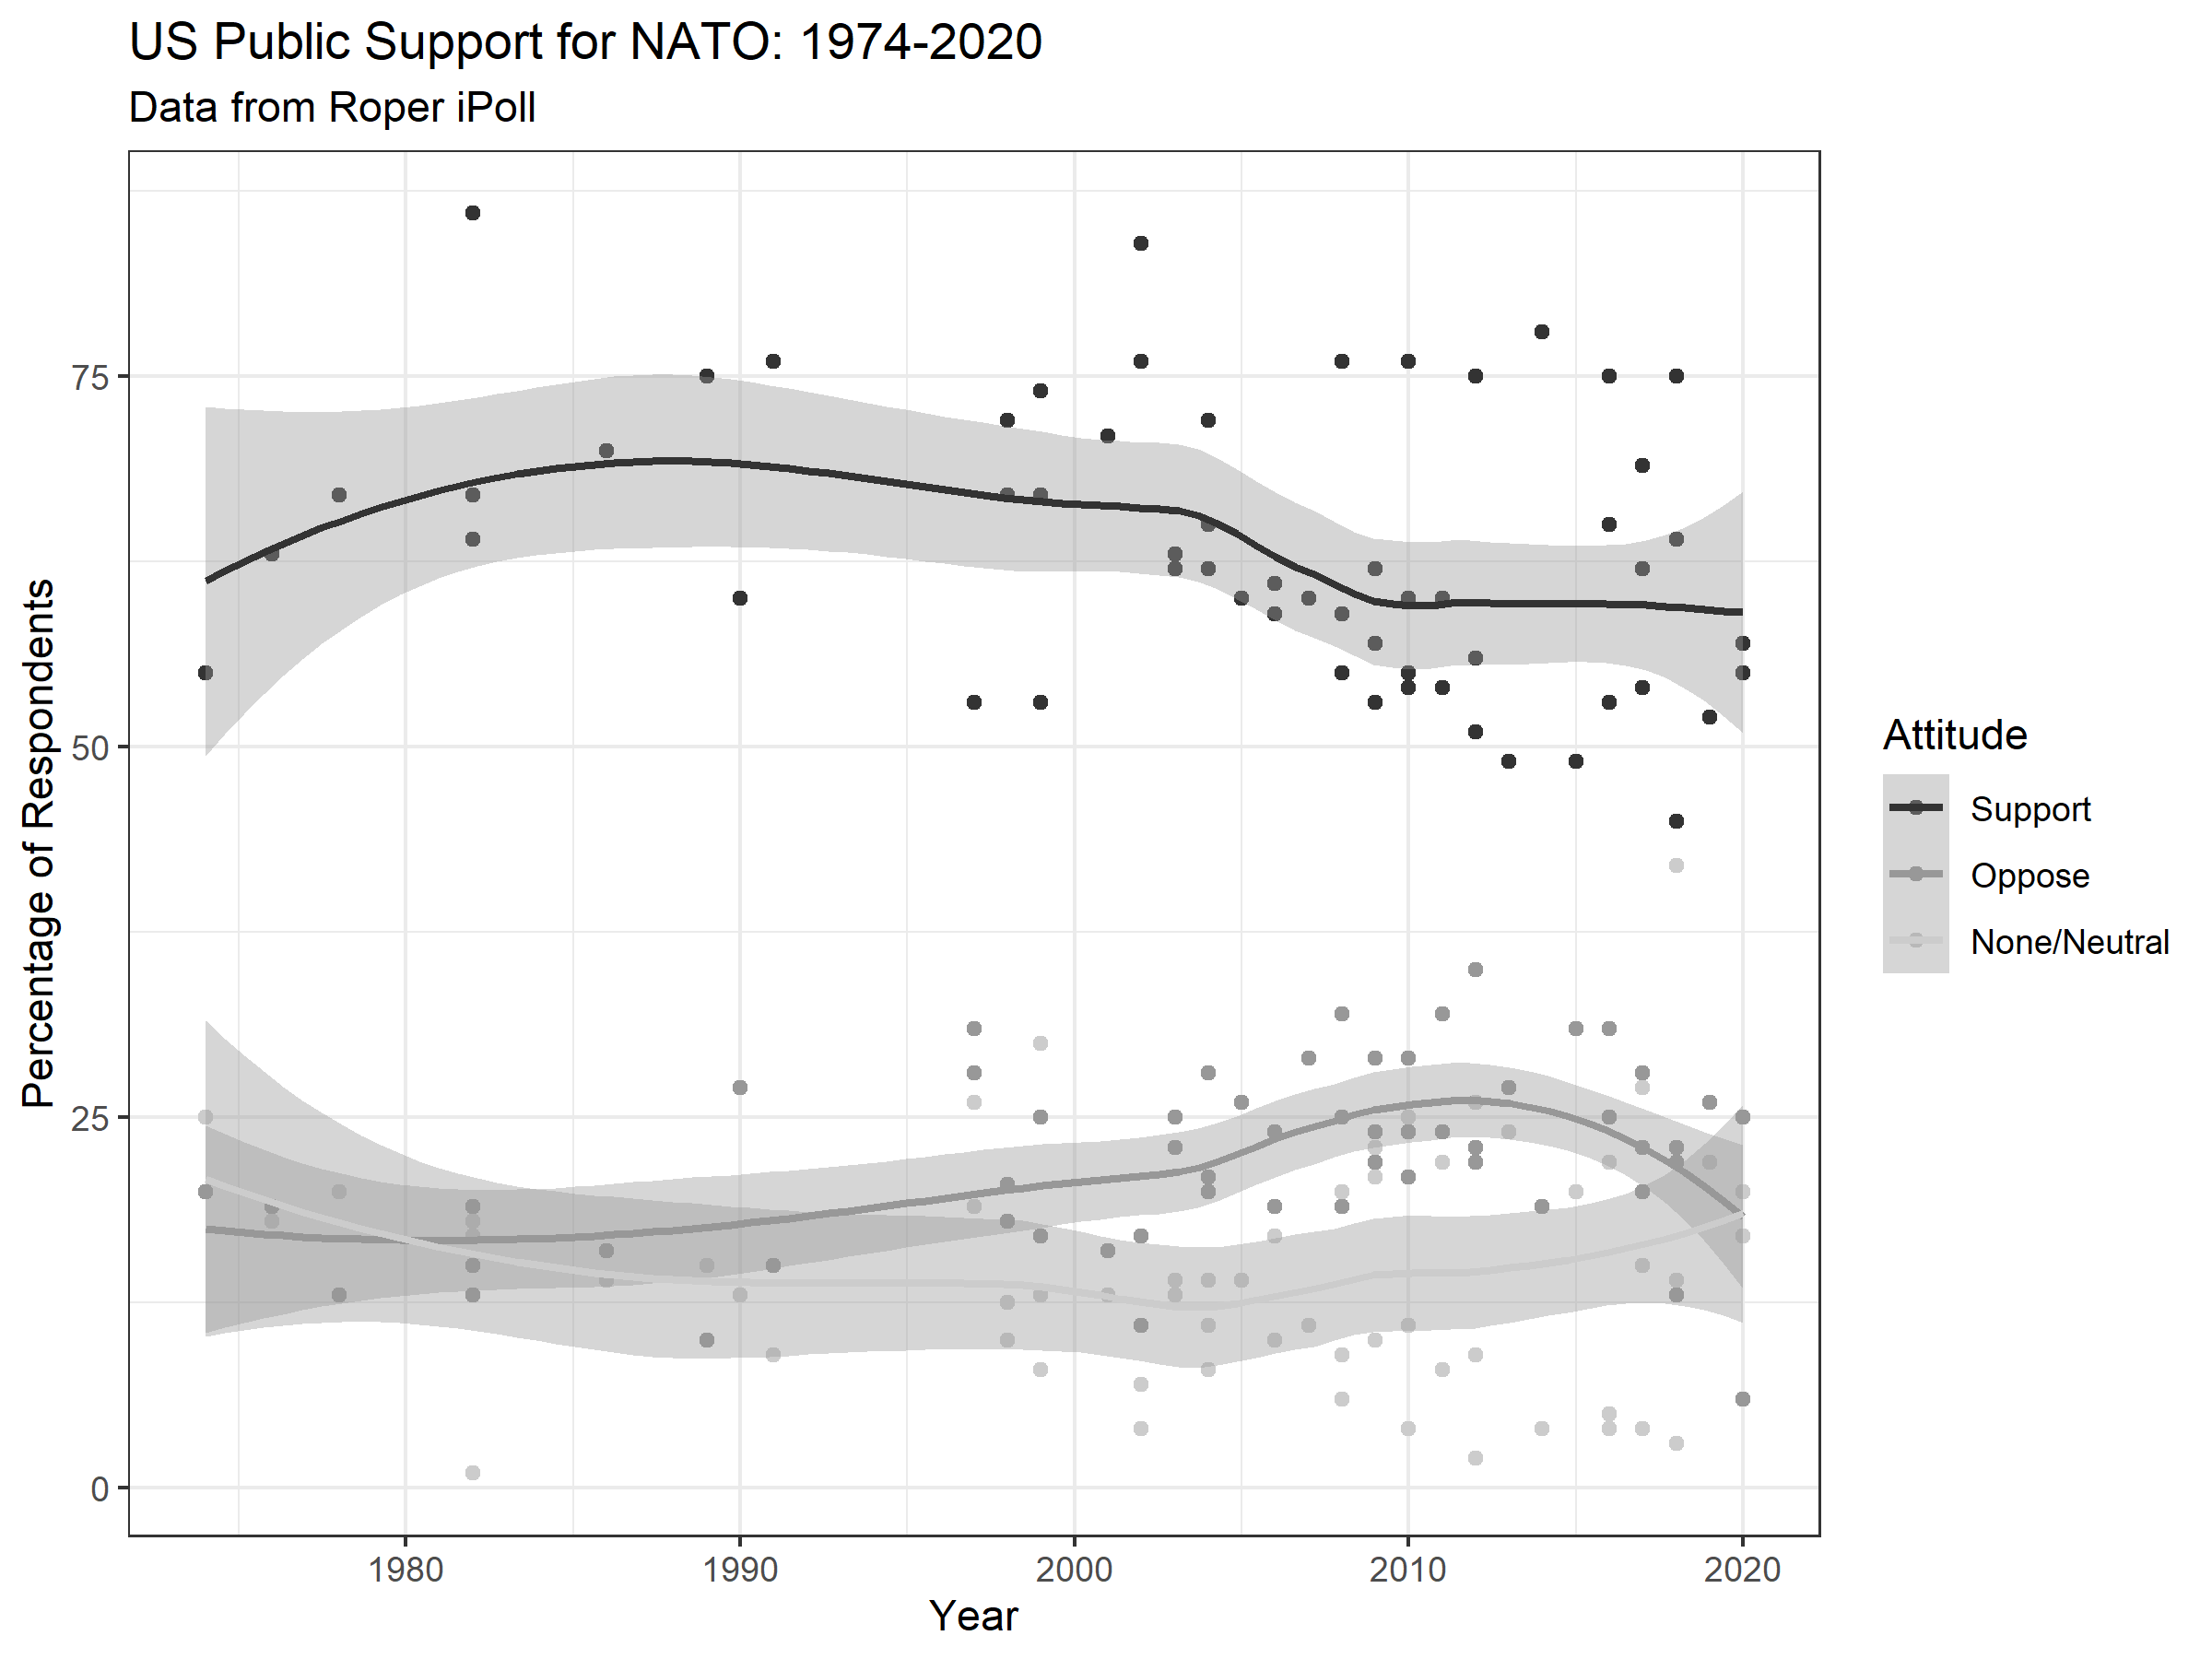
\includegraphics[width=0.95\textwidth]{../figures/nato-op-time.png}
	\caption{US public support for NATO from 1974 to 2020. Each point marks a unique poll, and colors differentiate the percentages of respondents that expressed support, opposition or neutral/no opinion of NATO. Loess lines estimate the average support for each group in every year. Topline data from the Roper Center's iPoll database.}
	\label{fig:nato-op-time}
\end{figure}


Are elite cues a viable explanation of the variation in alliance attitudes in \autoref{fig:nato-op-time}? 
The role of elite cues in observed alliance opinions is subject to a longstanding puzzle in public opinion on foreign policy.
When we observe elite and public support for alliances, it is unclear if public attitudes follow elite cues, only some of the public responds to elite cues or elite cues have little heft. 


Elite cues could exert extensive, conditional or minimal influence on alliance attitudes, and prior research suggests that all three possibilities are plausible. 
There is ample evidence for claims of extensive elite leadership of public opinion. 
For example, \citet{Canes-Wrone2006} finds that U.S. Presidents rarely follow public preferences they disagree with and have ample freedom to lead foreign policy attitudes. 
\citet{JacobsShapiro2000} argue that elites track public opinion to manipulate it, not conform to it.
Moreover, foreign policy is a secondary concern for many voters, so elite foreign policy views and rhetoric can diverge from public attitudes with few political repercussions \citep{BusbyMonten2012}.\footnote{\citet{Kreps2010} notes that public disapproval did not constrain participation in NATO's International Security Assistance Force in Afghanistan.}


Other findings suggest that elites conform their rhetoric and policy stances to public opinion, and thus have minimal influence. 
\citet{Barberaetal2019} use social media data to show that legislators are more likely to follow than lead public opinion, including on some foreign policy issues. 
\citet{HagerHilbig2020} find that exposure to public opinion research moves speech and policy positions by German politicians closer to majority opinion. 
\citet{Haesebrouck2019} uncovers little evidence that European elites led public support for military interventions in Libya and the Islamic State. 
%\citet{Bechteletal2015} find that elite cues and frames led Swiss individuals, especially those with low knowledge, to reinforce their prior immigration attitudes, rather than match elite cues. 
Even military elites who have no electoral concerns shape their policy recommendations in response to public opinion \citep{LinGreenberg2021}. 


Conditional elite influence is also possible. 
\citet{PageShapiro1992} note that public opinion is broadly consistent and rational, and changes in predictable ways in response to information from multiple sources, including elite cues. 
\citet{GuisingerSaunders2017} claim that for issues with low partisan polarization, information effects dominate public opinion, while elite cues matter more for polarized issues like cap and trade schemes.\footnote{\citet{GuisingerSaunders2017} map the boundaries of elite influence across issues. I build on this work by focusing on who responds to elite cues in alliance politics.}
Democrats express higher support for alliances like NATO than Republicans \citep{PewNATO2020} and this partisan gap in alliance attitudes falls in between polarized issues like the Iran nuclear program and more technical issues such as the International Criminal Court \citet{GuisingerSaunders2017}. 


Understanding alliance attitudes thus contributes to a fundamental debate about public opinion in foreign policy. 
In the following, I examine the extent of elite cues' influence on public opinion towards alliances.\footnote{I cannot fully address if elite cues follow public opinion, as I do not show what drives elite cues. Rather, I assess a crucial component of elite leadership that cannot be inferred from observational data.}
To do so, I analyze whether foreign policy dispositions change individual responses to co-partisan elite cues.
Predispositions towards using force and international engagement create distinct wings within the two major parties, and elite cues may reach most, some, or none of those groups.


Under extensive elite influence, most or all of the wings within U.S. parties respond to elite cues. 
Conditional elite influence where elite cues impact only half their party wings is also possible. 
Some alliance attitudes may be more plastic than others, given varying trust in elites. 
Finally, elite cues could have minimal influence, and reach one or no wings of their party.


The remainder of the argument starts by outlining the general process of elite cue leadership.
I then detail how partisanship and foreign policy dispositions determine baseline alliance attitudes and divide create foreign policy wings within parties.
Finally, I explain which responses to elite cues reflect extensive elite leadership. 


\subsection{Elite Cues} 
% Framing/elite leading


Elite cues models hold that the public follows trusted elites in forming their opinion, so elite portrayals of alliances bolster or undermine public support.
In this perspective, public opinion towards alliances permeates down from the top and is endogenous to elite views \citep{Druckman2014}.
There is substantial evidence that elites influence public foreign policy attitudes \citep{BaumPotter2008}. 
The media often convey elite cues, and social media may further amplify elite influence \citep{BaumPotter2019}.   


Elite support or opposition could shape alliance attitudes as individuals rely on trusted elites in an issue environment with little alternative information. 
Information shortcomings make individuals more responsive to elite framing and cues \citep{Druckman2001, Peterson2017} and the public lacks foreign policy information \citep{BaumPotter2008}.
This public response overcomes limited information by looking to perceived in-group elites. 
Alliance politics is a less salient foreign policy concern than many other issues, so elite cues may exert substantial influence.


% cue-giver matters 
Multiple elites give public alliance cues.
Elected officials, diplomats and military leaders all participate in alliance politics and are potential figures for public trust.
Political leaders' public visibility and influence is well-established.
Cues from military elites can shape public opinion about the use of force \citep{Golbyetal2018}, so military endorsements may also move alliance attitudes. 
Diplomatic elites are high profile experts.\footnote{Some diplomatic elites like the Secretary of State are political appointees, which complicates public interpretation of their cues. Even so, they have a distinct voice from other political elites.}
Public perceptions that military leaders and diplomats are well-informed about alliances will increase their influence, but some individuals may distrust these elites instead.


% highlight partisanship
In an elite cues model, support for alliances by trusted elites should increase individual support for alliances, and elite opposition will reduce support.   
Partisanship helps elites establish trust and makes co-partisan elite cues more influential \citep{Druckmanetal2013}.
Given partisan polarization, individuals distrust and discount messages from out-partisan elites.
As a result, unified elite cues create robust public support \citep{Berinsky2007}.


% transition paragraph: scope of influence
Elite cues are a straightforward and compelling explanation of alliance attitudes.
Even information about alliance characteristics like allied democracy or military spending likely reaches the public through elite rhetoric. 
This makes extensive elite influence on alliance attitudes plausible. 
The individuals who receive elite cues also hold prior attachments, intuitions and beliefs, however.
Foreign policy dispositions and partisanship could determine whether alliance attitudes change under elite cues by shaping who individuals trust within their party.


\subsection{Foreign Policy Dispositions and Partisanship}


% Overview para
Foreign policy dispositions and partisanship shape individual perceptions of international politics. 
These individual concerns modify the impact of elite cues by shaping which elites are in-group members.
Furthermore, they establish individuals' baseline alliance support, or willingness to back alliances in general, which creates differences in alliance attitudes between and within parties.\footnote{Another way to think of baseline support is an individual disposition to support an average or typical alliance.}
Within-party differences in foreign policy dispositions might change individual responses to co-partisan elite cues.
If individuals believe that elites are from a different party wing, they may discount elite cues.  
Should enough individuals hold prior attachments more tightly than partisan affiliations, elite cues will have minimal or conditional influence.


% foreign policy disposition
Foreign policy dispositions are intuitions about international politics \citep{KertzerTingley2018}. 
These principles shape how people respond to decisions such as backing down from military intervention \citep{KertzerBrutger2016}.\footnote{\citet{KertzerBrutger2016} leverage foreign policy dispositions to decompose audience costs into belligerence and consistency costs.}
Dispositions also set baseline inclinations towards alliances and shape affinity with party elites.
Whether and how individuals respond to elite cues given their prior dispositions shapes elite influence. 


% internationalists more likely
% Define internationalism  
Militant assertiveness and internationalism are two key foreign policy dispositions for alliance attitudes \citep{Herrmannetal1999}.\footnote{While internationalism and militant assertiveness are continuous concepts, I discuss them in categorical terms to maintain consistency with the experimental results, which require categorical disposition indicators.}
Internationalism is an inclination to engage with other countries and contribute to international endeavors. 
Internationalists support U.S. involvement in foreign affairs and are more likely to favor alliance commitments. 
Conversely, isolationists are skeptical of international institutions and cooperation, dislike foreign involvement and prioritize domestic affairs \citep{Kertzer2013}. 
Isolationist senators like Robert Taft were the core of U.S. opposition to ratifying NATO \citep{Kaplan2007}.
A U.S. tradition of discomfort with ``entangling alliances'' only broke after World War II \citep{Kupchan2020}.


% militant assertiveness 
Militant assertiveness reflects individual approbation of using force to address international problems \citep{Herrmannetal1999}. 
Dovish individuals with low militant assertiveness prefer nonviolent policies.
Hawks are more willing to employ force.
Although alliances are cooperative institutions, they also aggregate military capability and obligate members to fight.
General skepticism of using military force should make doves less likely to support military alliances that commit their country to fight.  
European pacifists are among the most consistent NATO opponents, for example \citep{Thies2015}.


Unlike doves, I expect that hawks value capability aggregation through alliances and are more willing to hazard foreign wars. 
Committing to fight for allies is also less problematic for hawkish individuals. 
In-group loyalty is a key source of militant assertiveness \citep{Kertzeretal2014} and should increase support for alliance participation by reinforcing group cohesion in the face of external pressures.


% no a priori about different combinations
There are four potential foreign policy dispositions around alliance attitudes.
Individuals may be isolationist and hawkish, internationalist and hawkish, isolationist and dovish, or internationalist and dovish.\footnote{While some existing research does not divide isolationists into hawks and doves, but distinguishes between cooperative and militant internationalists \citep{Kertzeretal2014}, I divide isolationists by hawkishness to assess the net impact of competing dispositions. To streamline discussion across the four categories, I do not use the terms cooperative and militant internationalism.}
The relative weight of overlapping dispositions on baseline attitudes is therefore an important concern. 
Dovish isolationists are the most likely alliance skeptics, while hawkish internationalists are the most likely alliance supporters. 
I do not have strong priors about the relative strength of hawkishness and isolationism, however.\footnote{As a result, parts of the following analysis are exploratory.}
One effect could dominate the other, the two factors could offset, or they could interact in unexpected ways.


% introduce/transition partisanship
% party wings
Partisanship and foreign policy dispositions interact to create differences in baseline alliance attitudes between and within parties. 
Party identification connects elite cues and individual concerns by determining which elite cues individuals trust.
Moreover, partisanship is correlated with militant assertiveness and internationalism. 
Conservatives in the United States have a longstanding history of isolationism \citep{Kupchan2020}.
Republicans are more hawkish than Democrats as well \citep{Gries2014}. 


% yet differences within parties
Differences in foreign policy dispositions across parties are well-known, but there is also substantial variation in foreign policy disposition within parties.
\citet{Dueck2019} divides Republicans into three foreign policy groups based on their attitudes towards international engagement and using force, for example.
Nonintervention Republicans abhor international engagement and using force.
Hawkish unilateralism reflects willingness to use force coupled with distrust of international entanglements. 
Last, conservative internationalists are more supportive of international engagement and using force abroad, though they retain some skepticism of multilateral institutions.


Democrats also have substantial internal foreign policy disagreements. 
Progressive Democrats favor multilateral international engagement, but are often more dovish.
Centrist Democrats are usually more hawkish, but still favor international engagement. 
The 2020 presidential primaries revealed disagreements between progressive Democrats like Bernie Sanders and Elizabeth Warren and centrists led by Joe Biden \citep{Robinson2019demfp}. 


% Similar dispositions, partisan differences
%Although foreign policy dispositions divide parties into competing wings on the same dimensions, parties are the primary in-group affiliation. 
%There are
%Republicans are often more concerned with national sovereignty, in particular. 
%Conservative internationalists and centrist Democrats share many foreign policy priorities, but disagree over how to pursue those ends.
%Centrist Democrats are more supportive of multilateral institutions than Republicans with similar foreign policy dispositions. 


% who influences
Within-party disagreements on foreign policy could constrain elite influence. 
Divergent dispositions may drive individual foreign policy disagreement with co-partisan elites.
If individuals believe that elites are not part of their foreign policy wing, they will neither trust elites nor follow their cues. 
As a result, elite cue influence may depend on shared foreign policy dispositions.


% elites face divided wings
Elite cue-givers in the United States do not send messages to a monolithic party.\footnote{Parties may have more unified foreign policy views in other electoral systems.}
Rather, elite cues reach different partisan wings, with potentially divergent consequences. 
Whether the in-group effect of partisanship overcomes out-group dynamics within parties is unclear. 


% limits 
Understanding alliance attitudes thus requires careful attention to elite cues, partisanship and foreign policy dispositions. 
Elite influence depends on whether elite cues move most, some, or none of the wings within each party. 
In the next section, I detail the three potential public responses to elite cues. 




\subsection{Assessing Elite Influence}


% how distinguished
To assess elite leadership, I examine how partisan elite cues impact Democrats and Republicans in the four wings of each party.
Partisanship, militant assertiveness and isolationism create distinct alliance attitudes within and between both parties. 
These inclinations set baseline alliance attitudes. 
How elite cues move attitudes relative to baseline opinions then shows who elites lead. 


If co-partisan elite cues impact three or more wings within their party, elites have extensive influence and lead most individuals regardless of foreign policy dispositions. 
When cues move attitudes in two of the four wings, cues exert conditional influence. 
Conditional influence suggests deep intra-party divisions over international engagement. 
Finally, minimal elite influence occurs when one or no wings heed elite cues.
Minimal influences suggests that elites are disconnected from their party's rank and file.


% dividing partisans
Dividing partisan respondents by foreign policy disposition thus provides leverage over who holds plastic or rigid alliance attitudes. 
Some individuals may trust their own party elites more. 
Especially when a wing falls outside a foreign policy consensus within their party, individuals in that group may discount elite cues.


% explain: isolation
Under extensive elite leadership, elite cues change public opinion with little reference to individual predispositions towards alliance participation. 
For example, co-partisan elite support will increase support for alliance participation even among some isolationists who disagree with many elites. 
Similarly, if elite opposition reduces support among hawkish individuals who would otherwise back an alliance, elite cues have extensive influence. 


% explain: hawks 
If elite cues have minimal or conditional impact, then intra-party disagreements constrain their influence.
Strong predispositions from isolationism and militant assertiveness could condition or minimize any direct impact of elite cues.
Elites might still exercise indirect leadership by shaping alliance salience and presenting specific information, but null or conditional effects correspond less with classic elite cues arguments. 


% table it here
\autoref{tab:arg-sum} summarizes these predictions. 
Extensive elite influence requires elites to move most or all of the potential wings in their party. 
Conditional influence takes place when elites reach half of the four groups. 
Finally, minimal influence means that elites reach one or none of the groups within a political party.


\begin{table}[hbt!]
\begin{center}
\begin{tabular}{| c | c | c | c |}
\hline
   Influence          & Extensive & Conditional & Minimal  \\
\hline
   Number of Wings   & \multirow{2}{*}{3 or 4}  & \multirow{2}{*}{2}  & \multirow{2}{*}{1 or 0} \\
   Following Elite Cues     &           &             &  \\
\hline
\end{tabular}
\caption{Criteria for assessing the extent of elite influence on alliance attitudes. There are four potential wings within each party with different combinations of hawkish or dovish and internationalist or isolationist foreign policy dispositions.}
\label{tab:arg-sum}
\end{center} 
\end{table}



% formation vs maintenance
Before discussing the research design, there are two important considerations. 
First, alliance formation and maintenance are distinct processes \citep{Snyder1997}. 
I therefore consider alliance formation and maintenance in separate survey experiments.
This assesses whether public views of new and existing alliance commitments diverge. 


% long-run cycles
Second, feedback between elite cues and public opinion is plausible in the long run. 
Perhaps public opinion shapes elite cues, which in turn alter public opinion. 
Elites could respond to growing alliance skepticism by encouraging opposition, or leading countervailing alliance support.
Such feedback takes time and would appear in longstanding alliances.
This paper can therefore establish part of a potential feedback cycle by identifying who responds to elite cues.  
If elites have conditional or minimal influence, feedback is more limited, however.
I now describe how I assess elite cues and alliance attitudes. 



\section{Research Design}



% justify conjoint: 
I unpack public support for forming and maintaining military alliances in the United States with two conjoint survey experiments. 
Information about observed alliances bundles elite support and alliance characteristics. 
Conjoint experiments allow researchers to decompose such composite phenomena and compare multidimensional treatments \citep{Hainmuelleretal2014}. 
%For example, \citet{BechtelScheve2013} assess how institutional design affects public approval for climate cooperation. 


% describe rating tasks
Both experiments employ a single-profile conjoint design with two dependent variables--- a binary indicator of support and a continuous rating of the alliance.\footnote{The results below use the binary support measure. Rating results give similar results; see the appendix for details.} 
I ask individuals to support and rate defensive military alliances with randomly generated profiles of alliance characteristics and elite cues. 
In the alliance formation experiment, I query respondents about five hypothetical new alliances. 
The alliance maintenance experiment presents five hypothetical existing alliances.


The experiments first measure key respondent characteristics.  
Individual pretreatment measures of partisanship, militant assertiveness and internationalism structure subgroup analyses examining how individual concerns shape baseline support for alliance participation and responses to experimental treatments. 
After measuring individual factors, I present a hypothetical alliance with a randomly generated profile of elite cues and characteristics in a table.\footnote{The appendix includes an example table and the exact outcome question wording.} 
Once respondents read the table, I ask them to rate the hypothetical alliance on a scale from 0 to 100 and express approval of alliance formation or maintenance with a yes/no question. 
I then present four more randomly generated alliance profiles so each respondent rates five hypothetical alliances.


% Add a table with conjoint attributes. 
The conjoint profile of each alliance partner draws from fourteen attributes, each with multiple levels. 
The attributes capture theoretically interesting alliance characteristics and generate plausible profiles.\footnote{There are no restrictions on value combinations in the alliance profiles. I employ this uniform randomization because all of these alliance profiles are plausible. This also generates crucial variation in elite cues.}
I randomize attribute order at the respondent level, so the table of attributes is consistent for each respondent. 
Drawing alliance profiles at random and providing multiple rating tasks in a conjoint experiment makes estimating the average marginal component effect (AMCE) for each alliance attribute straightforward \citep{Hainmuelleretal2014}. 


\begin{table}
\begin{adjustbox}{width = .99\textwidth}
\begin{tabular}{lc} 
\hline \\ 
\textbf{Attributes} & \textbf{Values} \\
\hline \\ 
Republican Senators & Support an alliance with this country. \\
                    & Oppose an alliance with this country. \\ 
                    
Democratic Senators & Support an alliance with this country. \\
                    & Oppose an alliance with this country. \\ 
                    
The Joint Chiefs of Staff & Support an alliance with this country. \\
                    & Oppose an alliance with this country. \\ 
                    
The Secretary of State & Supports an alliance with this country. \\
                    & Opposes an alliance with this country. \\ 
                    
Trade Ties          & The United States has minimal trade ties with this country. \\
                    & The United States has modest trade ties with this country. \\
                    & The United states has extensive trade ties with this country. \\ 
% modified from Tomz and Weeks 2013 APSR: https://web.stanford.edu/~tomz/pubs/TomzWeeks-2013-11-Appendix.pdf 
Partner Political Regime    & This country is not a democracy, and shows no sign of becoming a democracy. \\
                    & This country is a democracy, but shows signs that it may not remain a democracy. \\ % democ backsliding
                    & This country is a democracy, and shows every sign that it will remain a democracy. \\
                    
Partner Military Capability & 10,000 soldiers and spends 1\% of their GDP on the military. \\ % low
                    & 80,000 soldiers and spends 2\% of their GDP on the military. \\ % moderate
                    & 250,000 soldiers and spends 3\% of their GDP on the military. \\ % high 
                    
Shared Threat       & The United States and this country face minimal common threats. \\ 
                    & The United States and this country face modest common threats. \\
                    & The United States and this country face serious common threats. \\
                    
Recent Military Cooperation  & This country has not participated in recent U.S. military operations. \\ 
                    & This country recently supported U.S. airstrikes against terrorists. \\
                    & This country recently supported U.S. counterinsurgency operations. \\
                    & This country recently fought with the United States in a war. \\
                    
Financial Cost      & This alliance requires \$5 billion in annual U.S. defense spending.  \\ 
                    & This alliance requires \$10 billion in annual U.S. defense spending.  \\ 
                    & This alliance requires \$15 billion in annual U.S. defense spending.  \\ 
                    
Conditions on Support  & The alliance treaty promises military support in any conflict. \\ 
                    & The alliance treaty promises military support only if this country did not provoke the conflict. \\ 
                    & The alliance treaty promises military support only if the conflict takes place in this country's region. \\
                    
Defense Cooperation & None. \\ 
                    & The alliance treaty provides basing rights for U.S. troops. \\
                    & The alliance treaty includes a shared military command. \\
                    & The alliance treaty includes an international organization to coordinate defense policies.  \\ 
% Issue linkages                    
Related Cooperation & None. \\
                    & The alliance is linked to greater trade and investment with the United States. \\ 
                    & The alliance is linked to greater support for the United States in the United Nations. \\ 
                    
Region              & Europe. \\ 
                    & Africa. \\
                    & The Middle East. \\ 
                    & Asia. \\   
                    & The Americas. \\ 
                                                                            
\hline \\
\end{tabular}
\end{adjustbox}
\caption{Table of alliance attributes in conjoint experiment profiles. The alliance formation and maintenance experiments both use all these attributes.} 
\label{tab:conjoint-vars}
\end{table}


% summarize table
The alliance profiles include many salient attributes, which I detail in \autoref{tab:conjoint-vars}. 
Support or opposition from Republican and Democratic Senators, the Joint Chiefs of Staff, and the Secretary of State provides elite cues from elected officials, military leaders and diplomats. 
Independent randomization of elite cues helps differentiate which elites are most influential.


Media reports often include other information besides elite cues \citep{BaumPotter2008}, so the experiments also present many alliance characteristics. 
I include key alliance characteristics such as trade ties \citep{Fordham2010}, regime type, shared threat, military capability \citep{Johnsonetal2015}, conditions on support, defense cooperation \citep{Morrow1994, LeedsAnac2005}, and issue linkages \citep{Poast2012}.
All of these factors shape perceived alliance value. 
A regime type indicator includes nondemocracy, fragile democracy, and consolidated democracy, as individuals may believe that democracies should cooperate because they share common concerns and values \citep{Chuetal2021}. 
The financial costs reflect a rough association between an alliance commitment and U.S. military spending from \citet{AlleyFuhrmann2021}. 
Recent military cooperation can bolster a partner's reputation \citep{Crescenzietal2012, GannonKent2020}.
I also randomize the region of the hypothetical alliance partner to mitigate confounding on other dimensions like cultural similarity.


Using hypothetical alliances creates general results through random assignment of crucial country and alliance characteristics. 
Meaningful experimental variation permits inferences about elite cues and allied characteristics that are fixed in many observed alliances.\footnote{While this raises potential confounding concerns, the regional indicator should limit confounding on other dimensions.}
Accounting for many alliance characteristics reduces the likelihood that any impact of elite cues is driven by inferred alliance characteristics.
It also mimics media presentations that bundle elite cues and information about an alliance. 
With fourteen unique alliance characteristics, the conjoint experiments give a detailed portrait of each alliance.


% Justify number of attributes
Including fourteen attributes for each hypothetical alliance also ensures that attributes do not mask one another without respondents feeling overwhelmed and reducing their effort in assessing the full profile.
Studies of satisficing in conjoint experiments suggest that including fourteen attributes in a profile is unlikely to reduce data quality \citep{Bansaketal2019}. 
Furthermore, there is little evidence of satisficing when researchers ask subjects to rate or compare five profiles \citep{Bansaketal2018}.



\subsection{Sample and Individual Measures}


Two separate experiments address alliance formation and maintenance. 
Each sample contains 1,500 U.S. respondents, recruited through Lucid Theorem, which approximates a representative sample through quota sampling.
\citet{CoppockMcClellan2019} find that this platform provides a solid approximation of demographic and experimental results in other contexts, and note that convenience samples like this are a good fit for estimating experimental treatments for the population of U.S. adults.
With an effective sample size of 7,500 from 1,500 respondents completing five rating tasks, the estimates will be under powered for very small effects, but should have enough power to pick up large differences and treatment interactions. 


I measured key individual correlates of alliance attitudes for each respondent, focusing on party affiliation\footnote{I classified independent ``leaners'' as Democrats or Republicans, respectively. I coded pure independents or others who expressed no partisan lean as independents.} and foreign policy dispositions. 
I used standard questions to measure internationalism and militant assertiveness \citep{KertzerBrutger2016}.
Analyzing subgroups in conjoint experiments requires categorical measures of foreign policy dispositions and partisanship.
I divided respondents into isolationists and internationalists by coding agreement with a common survey measure of isolationism as isolationism and disagreement or a neutral stance as internationalism. 
The hawkishness index sums three questions about the use of force and war. 
Hawks scored above the midpoint of three on this scale, while doves scored three or lower. 
Finally, I interacted party affiliation, hawkishness and isolationism to analyze foreign policy dispositions within partisan groups.\footnote{The appendix summarizes the distribution of foreign policy dispositions within the parties.} 


The analysis starts with unconditional average marginal component effects (AMCEs).
This establishes the aggregate impact of elite cues. 
After that, I explore elite influence by examining how partisanship and foreign policy dispositions modify the impact of elite cues. 
To analyze alliance support in the party wings, I estimate the overall mean choice for each group, then compare it to the marginal means of support under each attribute level.
Marginal means capture average choices or ratings for each conjoint attribute level, averaging over all other treatments. 
I also estimate omnibus F-tests \citep{Leeperetal2020} that find clear differences between the subgroups.  


\section{Results} 


Elite cues exert extensive but incomplete leadership over alliance attitudes.
The precise consequences of elite cues depend on partisanship and foreign policy dispositions because in addition to wide variation in baseline alliance support, a few affiliates of both parties hold rigid opinions. 
First, \autoref{fig:joint-plot} presents the AMCEs of elite cues on individual support choices in the alliance formation and maintenance experiments.\footnote{To facilitate presentation of the findings, all results figures show elite cues estimates. See the appendix for alliance characteristic results.}


The unconditional AMCE estimates suggest substantial elite influence on alliance attitudes. 
Elite cues increase public support for alliance formation and maintenance. 
The partisan elite support AMCEs are the largest such estimates in both experiments.
Partisan elite cues are therefore a salient influence on alliance attitudes for at least some respondents. 


Other elite cues also impact overall support for alliance participation. 
Public attitudes respond to cues from military leaders nearly as much as partisan elites, which is unsurprising given widespread public deference to the military \citep{Golbyetal2018}. 
Backing from the Secretary of State increases support for alliance formation and has a small positive effect on alliance maintenance choices. 
Less deference to bureaucrats and inferred partisan affiliations could explain limited influence by the Secretary of State. 
Moreover, individuals may expect the State Department to advocate for international engagement, especially existing partnerships.


\begin{figure}[htpb]
	\centering
		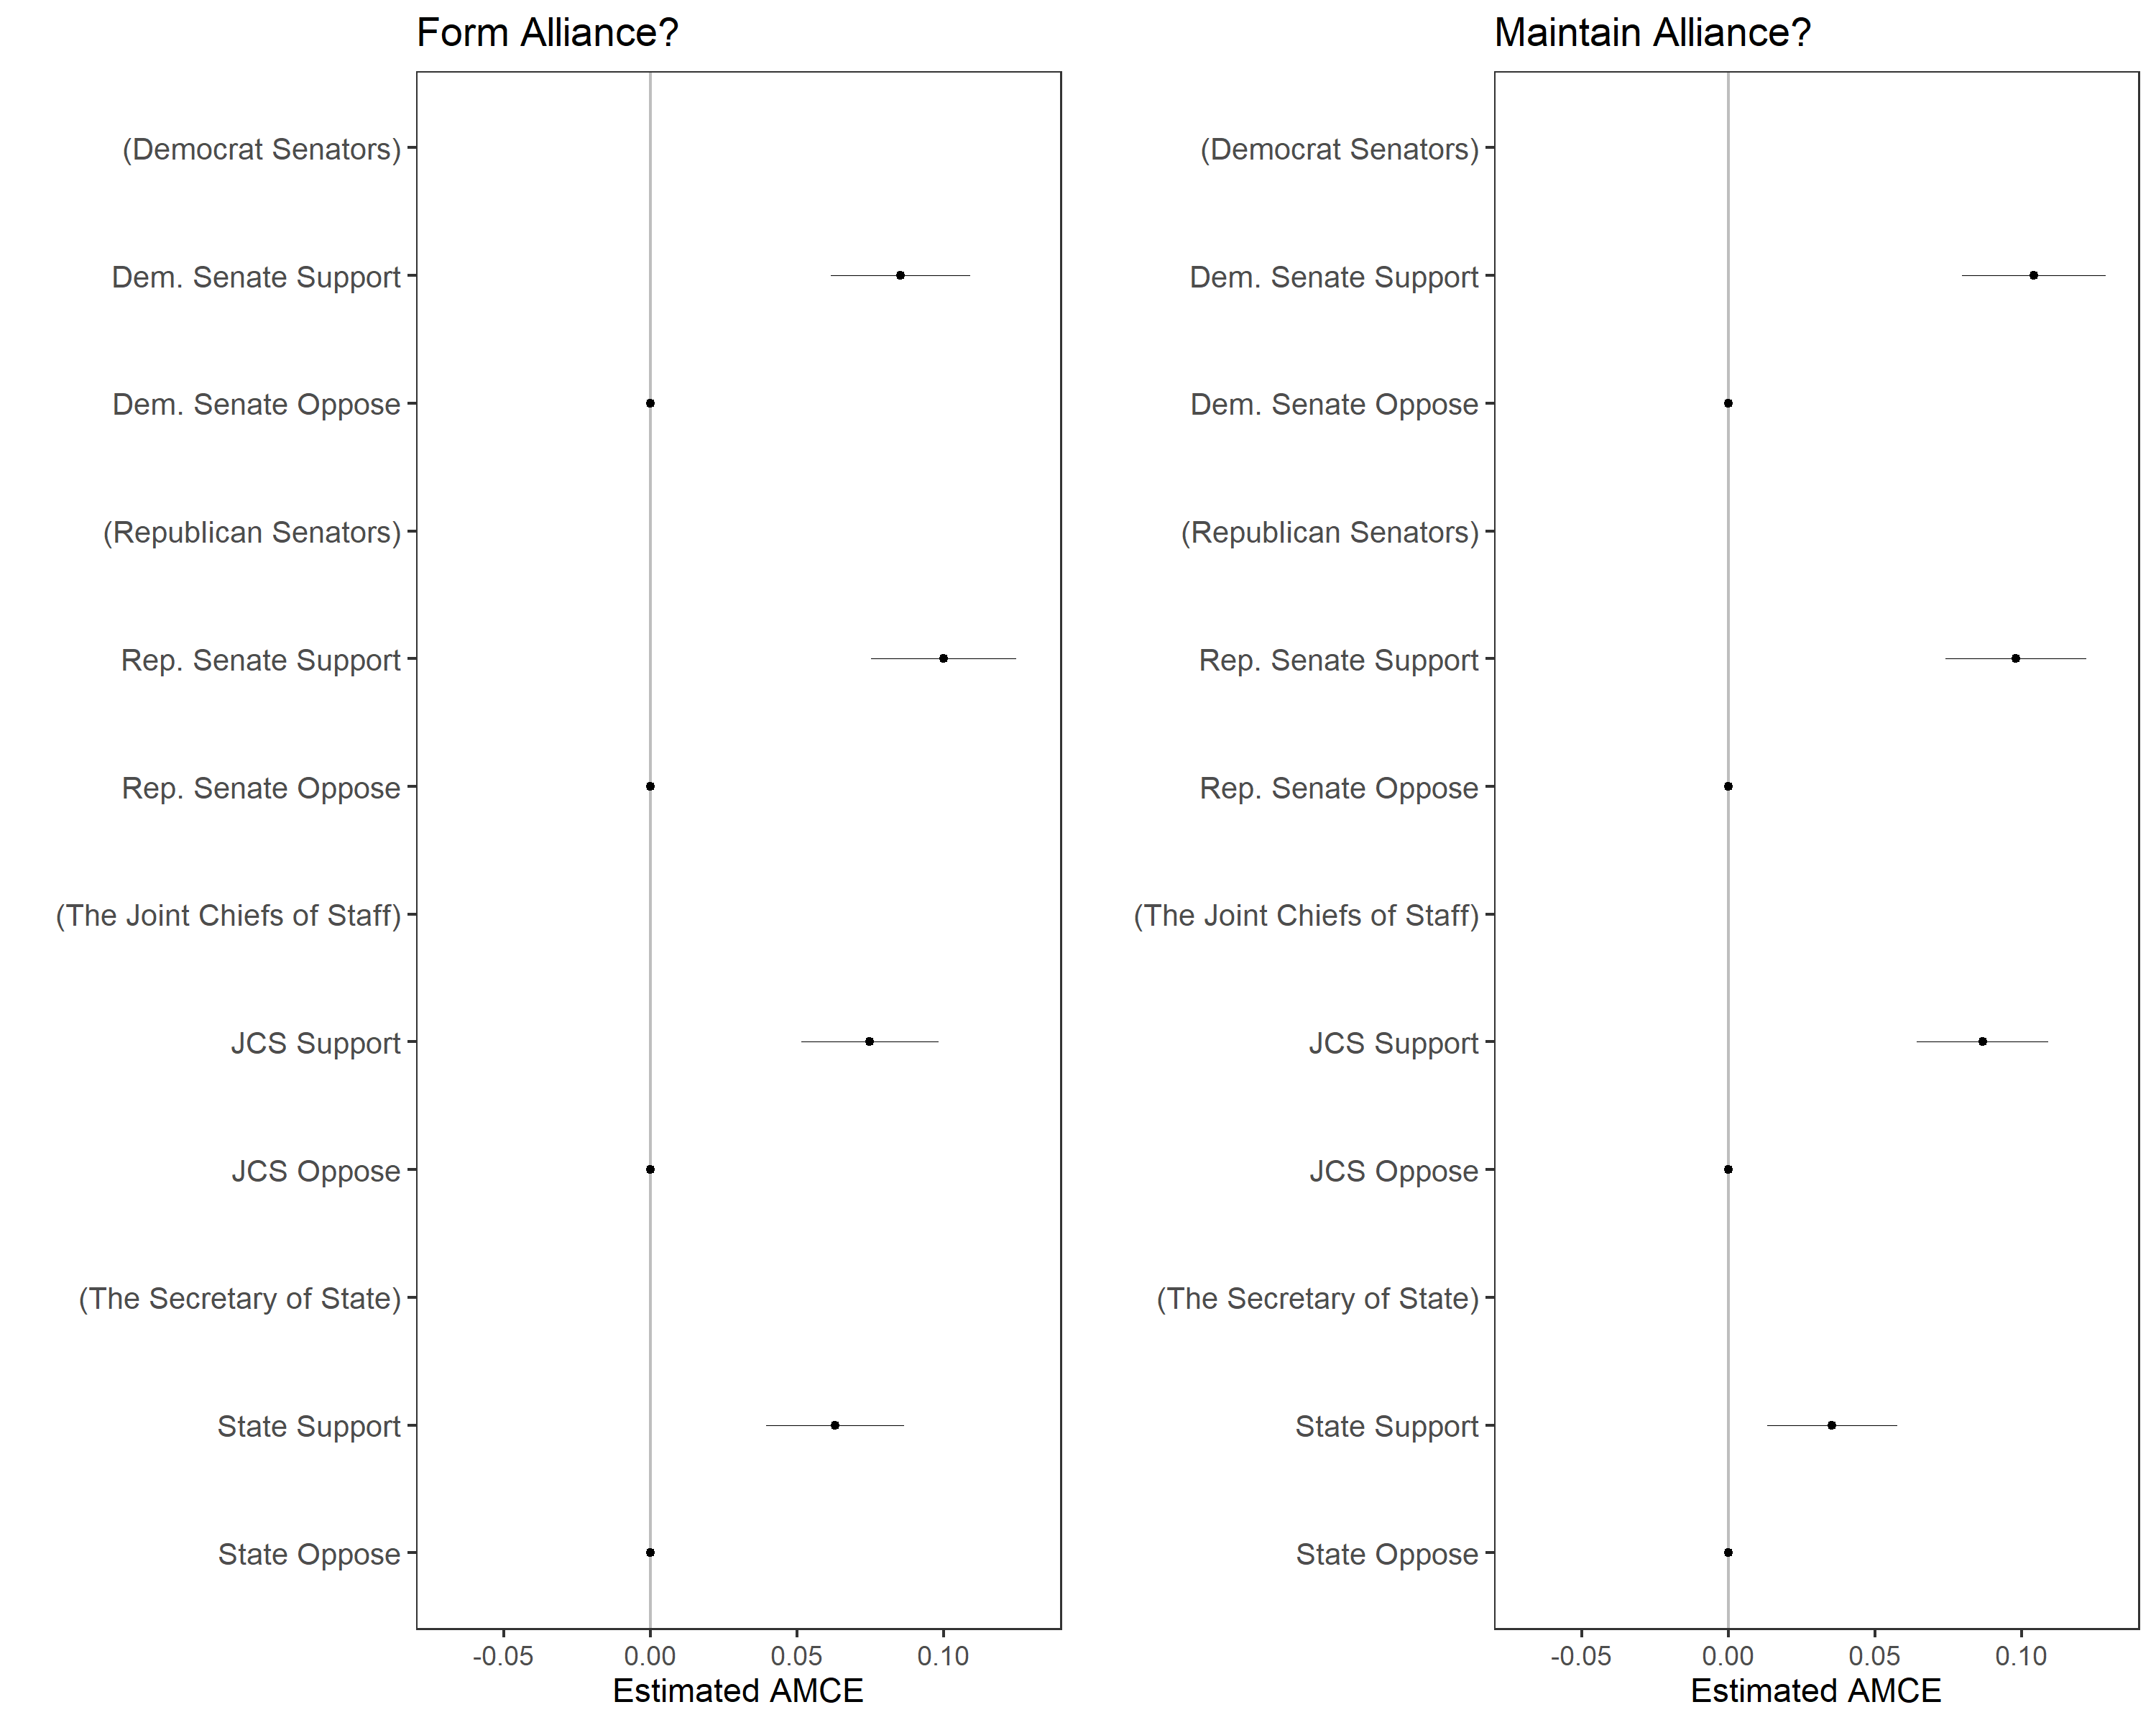
\includegraphics[width=0.95\textwidth]{../figures/joint-amce-plots-el.png}
	\caption{Average marginal component effect of elite cues on public support for forming or maintaining a hypothetical military alliance. Feature names in parentheses. Estimates with a dot at zero are the base attribute level. Components marked with abbreviated labels and all alliance characteristic attributes omitted to make the plot more legible.}
	\label{fig:joint-plot}
\end{figure}


The average effects in \autoref{fig:joint-plot} ignore differences in partisanship and foreign dispositions.
These estimates suggest that elites have some influence, but do not show the extent of elite influence within each party. 
The next estimates address this issue and establish which wings of the Democratic and Republican parties follow elite cues. 


\autoref{fig:party-dispo-form-el} and \autoref{fig:party-dispo-main-el} show the marginal means of support for alliance formation and maintenance from elite cues across party wings.
Each panel plots the marginal mean of support for each elite cue within every categorical combination of militant assertiveness, internationalism and partisanship.
The solid vertical line in every facet marks a marginal mean of .5 and a dashed line summarizes the average alliance choice across all attributes and levels for that group.
The average choice in all experimental conditions and tasks establishes a rough baseline attitude in each group.  


There are three key findings in \autoref{fig:party-dispo-form-el} and \autoref{fig:party-dispo-main-el}. 
First, co-partisan elite cues influence three of the four wings in both parties, which is consistent with extensive elite influence. 
Second, one wing of each party holds rigid alliance attitudes because they are outside their party's foreign policy mainstream.  
Finally, support for alliance maintenance is more rigid than support for alliance formation, perhaps because extant commitments activate moral considerations \citep{TomzWeeks2021}. 


\begin{figure}[htpb]
	\centering
		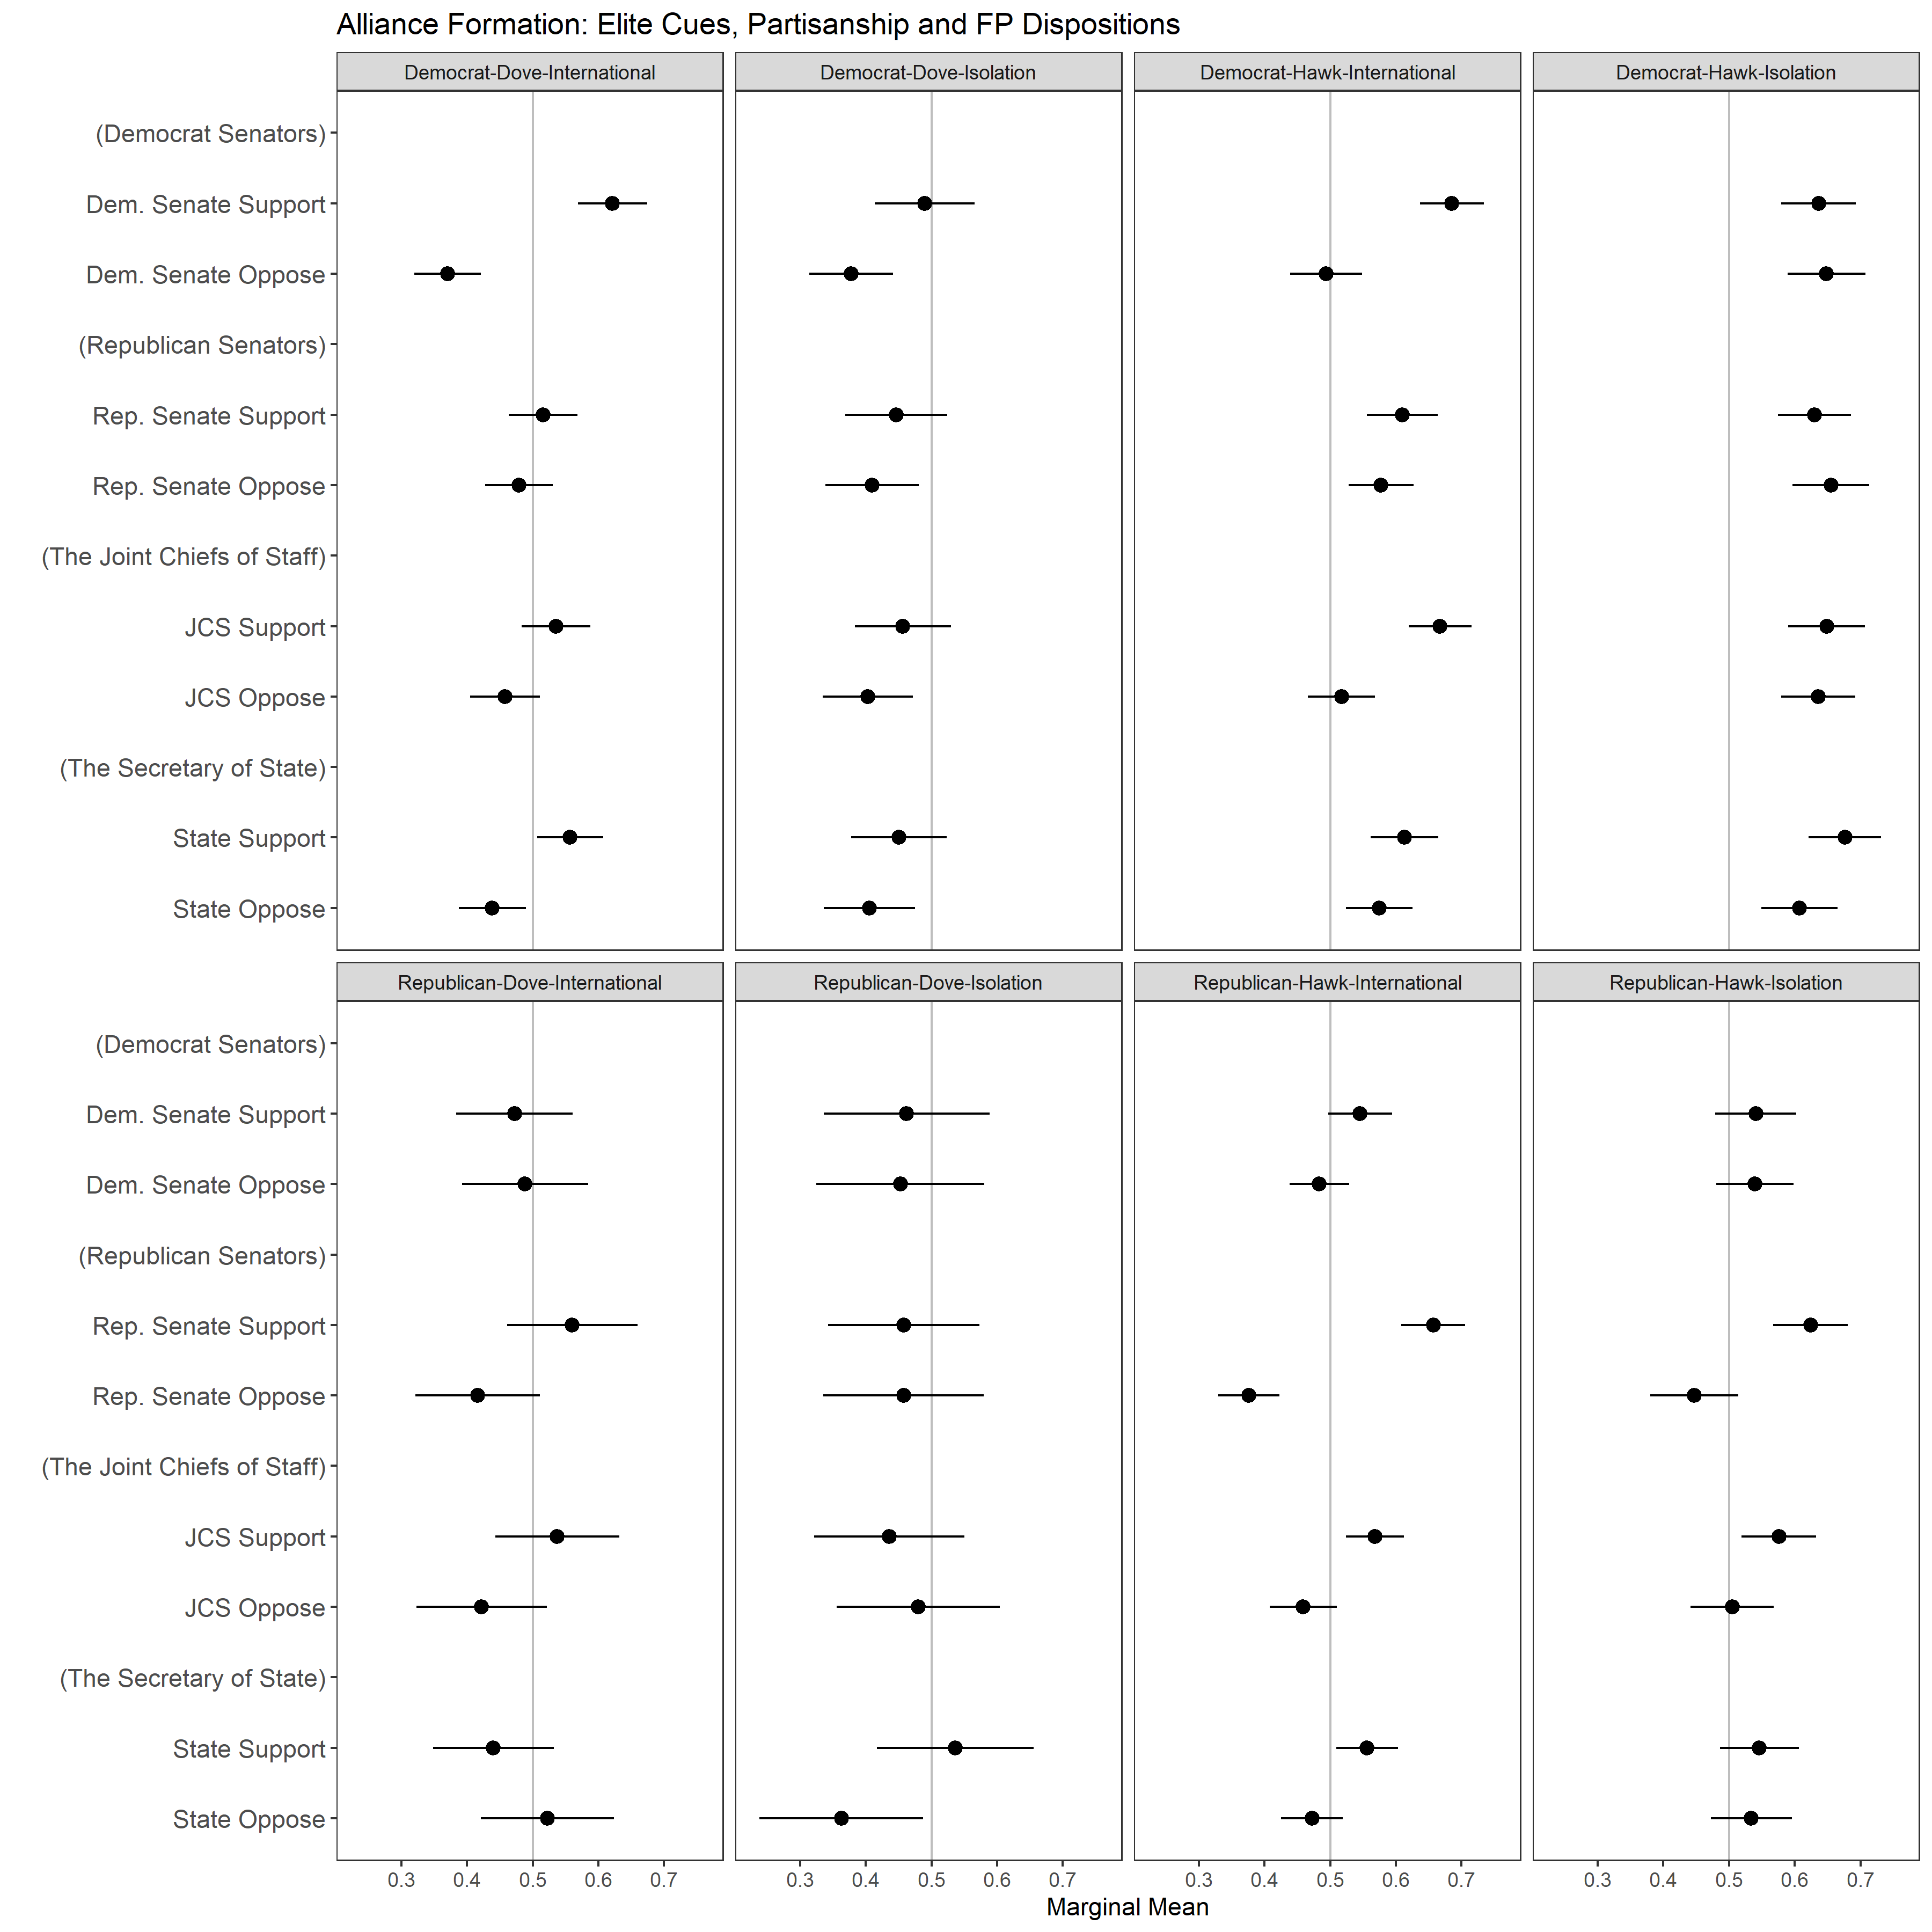
\includegraphics[width=0.95\textwidth]{../figures/party-dispo-form-el.png}
	\caption{Marginal means of support for forming hypothetical alliances across party identification and foreign policy dispositions given different elite cues. For each group, the estimates mark the marginal mean of support for alliance participation under different alliance treatments. The solid vertical line highlights a marginal mean of .5, while the dashed line marks the average choice across all levels. Components given abbreviated labels to make the plot more legible. Independents omitted.}
	\label{fig:party-dispo-form-el}
\end{figure}


Foreign policy dispositions produce substantial differences in alliance attitudes between and within parties. 
Among Democrats and Republicans, hawkishness increases general support for alliance participation.
Hawkish Democrats express higher support for alliance participation than hawkish Republicans, however. 
Willingness to use force encourages support for security cooperation. 
Internationalism offsets part of the negative impact of dovish dispositions on alliance support. 


Isolationists are more skeptical of alliances, but hawkishness generally outweighs skepticism towards international engagement in alliance attitudes. 
Isolationist and hawkish Democrats are the strongest alliance supporters. 
In the Republican party, isolationist hawks are far more supportive of alliances than isolationist doves.
The central role of in-group loyalty in hawkish dispositions \citep{Kertzeretal2014} is the most likely explanation of hawks' robust alliance support. 


\begin{figure}
	\centering
		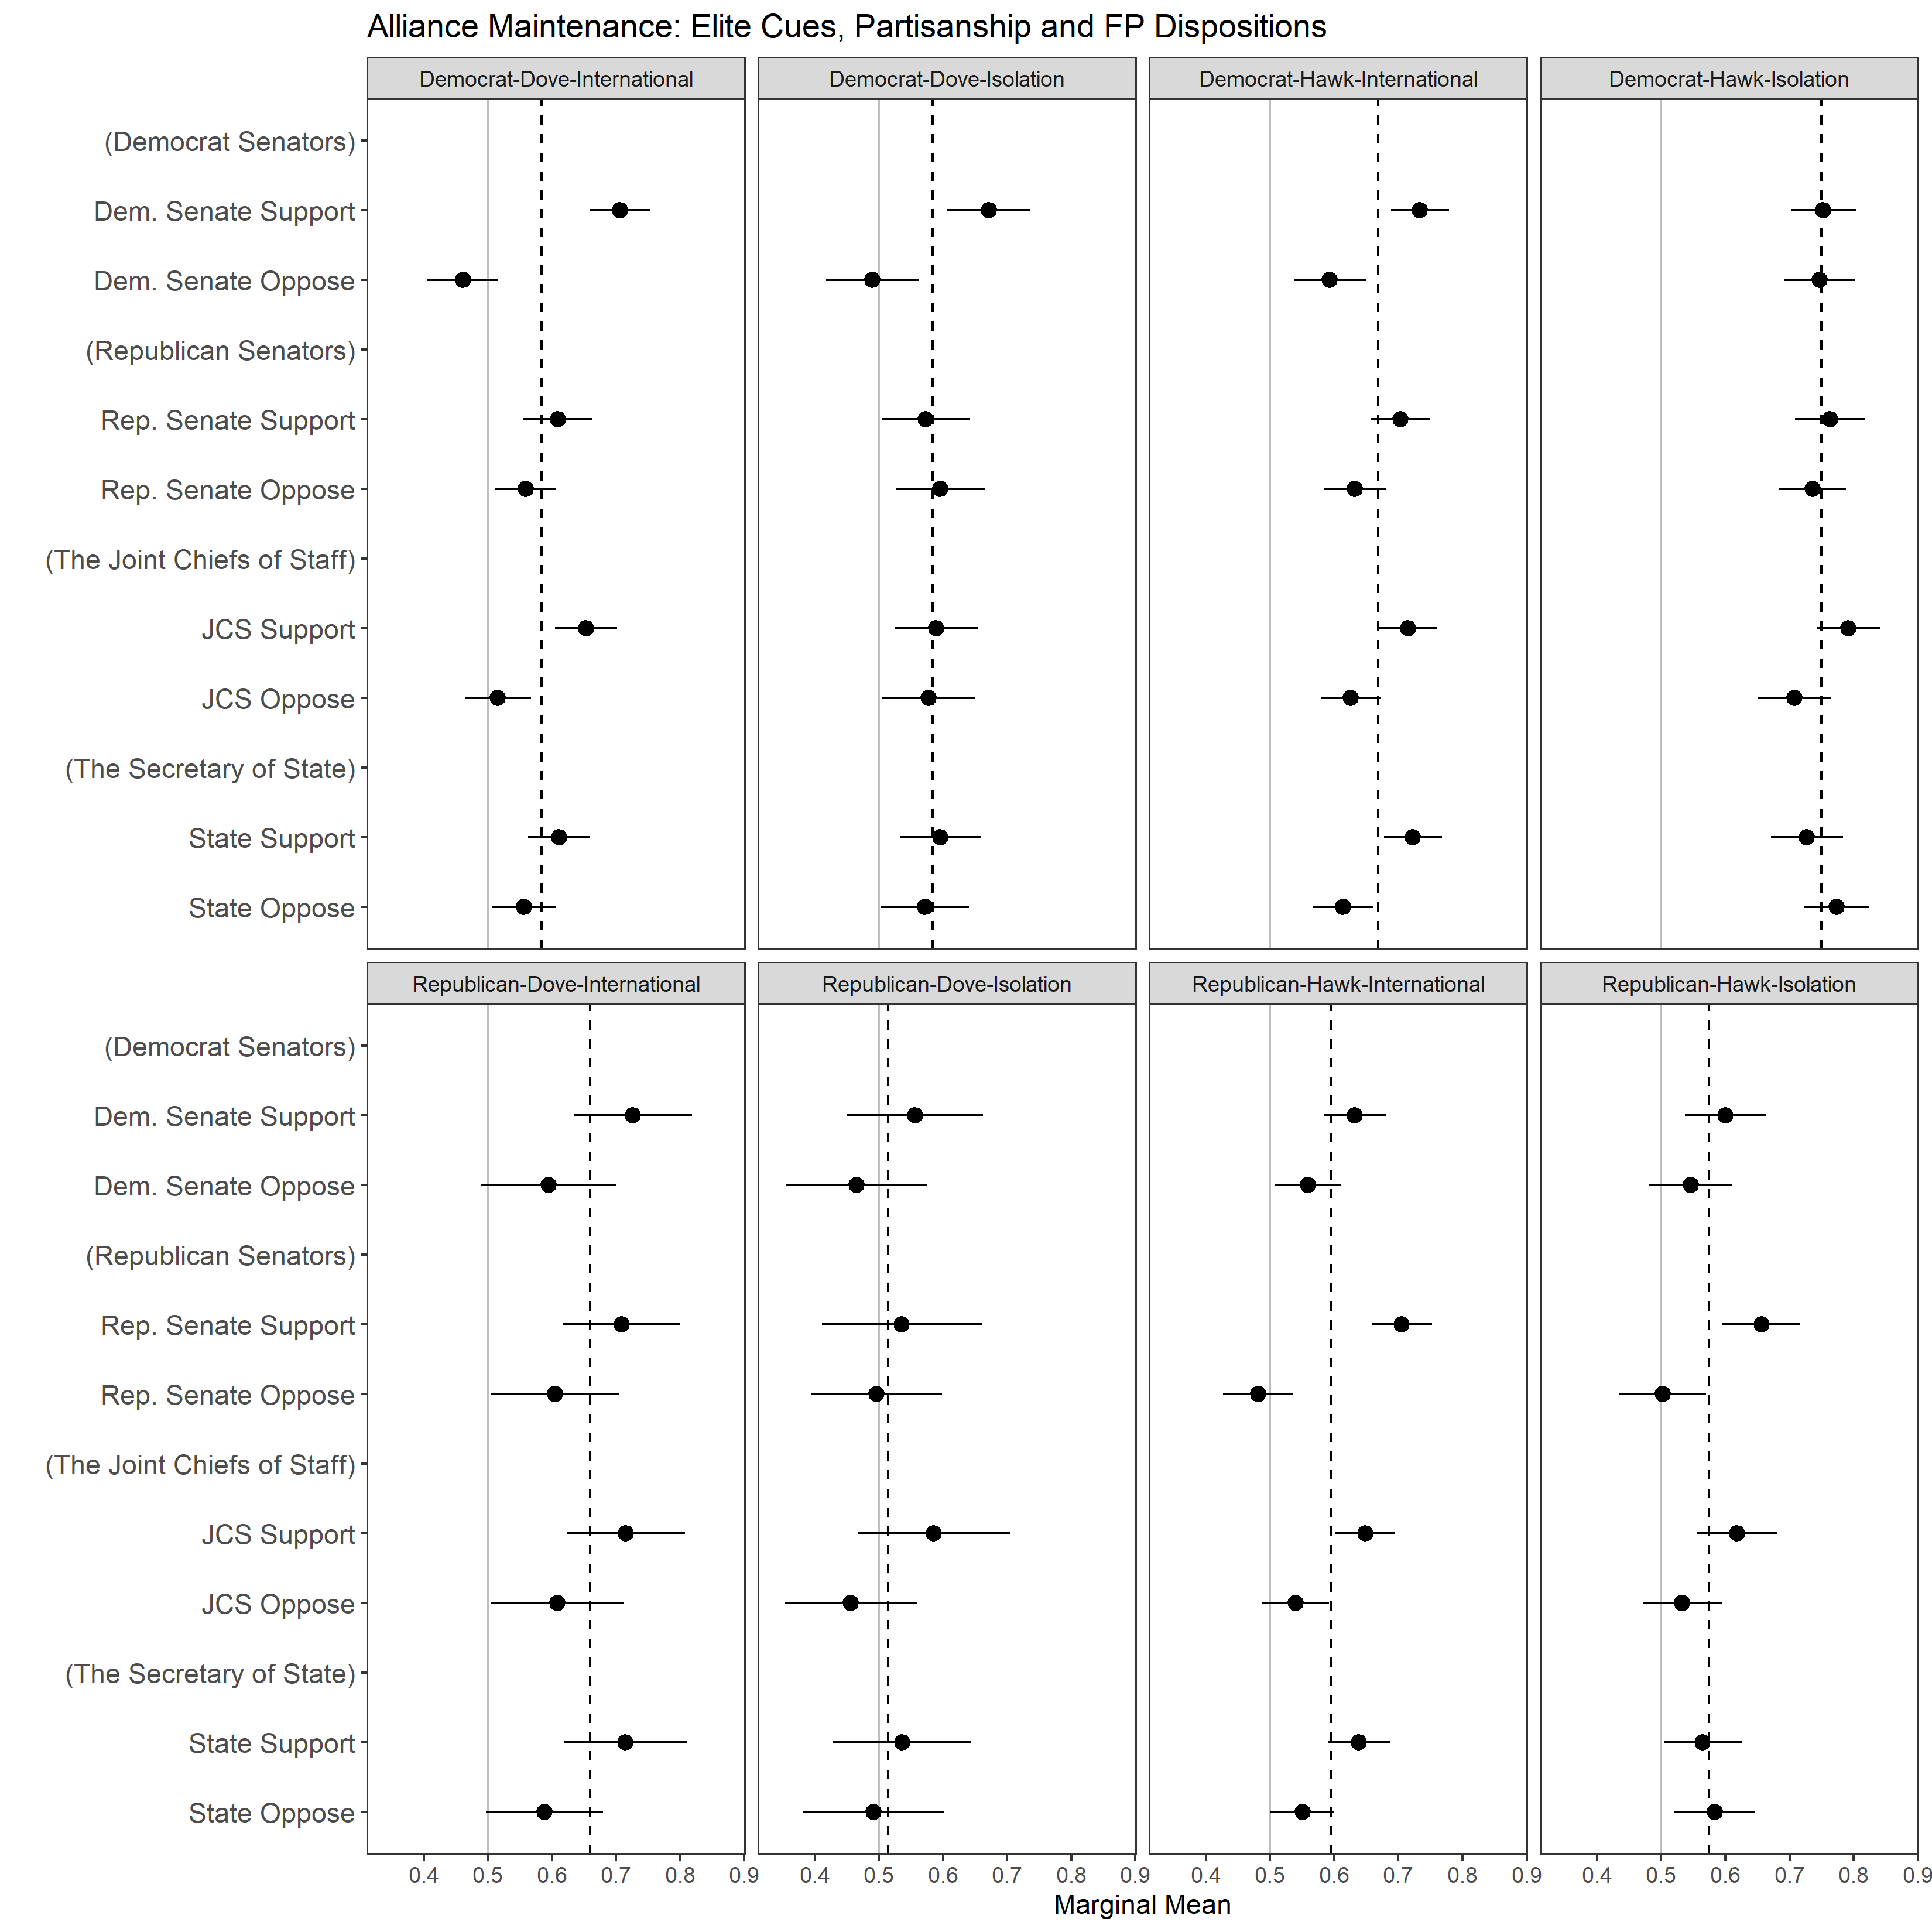
\includegraphics[width=0.95\textwidth]{../figures/party-dispo-main-el.png}
	\caption{Marginal means of support for maintaining hypothetical alliances across party identification and foreign policy dispositions given different elite cues. For each group, the estimates mark the marginal mean of support for alliance participation under different alliance treatments. The solid vertical line highlights a marginal mean of .5, while the dashed line marks the average choice across all levels. Components given abbreviated labels to make the plot more legible. Independents omitted.}
	\label{fig:party-dispo-main-el}
\end{figure}


The strongest alliance opponents are skeptics of international engagement and using military force. 
Isolationist and dovish individuals are least likely to support alliance formation and maintenance, as they lack any inclination to support capability aggregation via international cooperation.
Although few Republicans are doves, they are integral to alliance skepticism in the Republican party, especially when they also hold isolationist views.
Dovish Democrats are also more likely to oppose alliance participation.  


In addition to shifting baseline alliance attitudes, foreign policy dispositions change individual responses to elite cues. 
Internationalist Democrats respond to support from Democratic Senators, and also follow cues from the Secretary of State and Joint Chiefs of Staff. 
Hawkish and isolationist Democrats express consistent high support for forming and maintaining alliances regardless of partisan elite cues, though they may heed military elite cues on alliance maintenance. 
The strongest alliance supporters in the Democratic party thus hold rigid alliance attitudes.


It is somewhat counter-intuitive that hawkish and isolationist Democrats are the strongest alliance supporters. 
The most likely explanation of this is that isolationism has distinct meanings within different parties.
Calls to emphasize domestic over international concerns likely have different implications for Democrats and Republicans.
Future research should also check this finding with alternative isolationism scales. 


Among Republicans, hawks respond to elite cues, as most Republican elites are hawkish themselves. 
Regardless of their view of international engagement, there are clear differences in alliance support for hawkish Republicans based on Republican Senate support or opposition.
Hawkish Republicans also follow cues from military elites, and internationalist hawks in the GOP further look to diplomatic leaders. 
As a result, Republican elites lead alliance attitudes among individuals who are disposed to support forceful international engagement, so their opposition constrains alliance support among the most likely alliance backers in their party. 
The change in hawkish Republican attitudes from Republican elite cues is especially pronounced in the alliance formation experiment. 
Dovish and isolationist Republicans pay little attention to elite cues. 
The most consistent alliance opponents in the Republican party hold rigid alliance attitudes, which is the reverse of the Democratic party. 


% little bit on why
Out-group dynamics from foreign policy dispositions \textit{within} parties explain the asymmetric partisan rigidity in alliance attitudes. 
Isolationist, hawkish Democrats and dovish, isolationist Republicans hold opposite alliance attitudes, but they are both outside the mainstream in their party.
Isolationism and hawkishness places some Democrats outside the more dovish and pro-engagement core of the Democratic party. 
Dovish isolationism diverges from the hawkish mainstream of Republican politics as well. 
These two groups therefore treat co-partisan elites as out-group members.  


% group size
Rigid alliance attitudes are rare in these samples.
In the alliance formation experiment, 7\% of Republicans and 25\% of Democrats hold foreign policy dispositions that limit their response to co-partisan elite cues. 
In the alliance maintenance experiment, 9\% of Republicans and 23\% of Democrats have similarly rigid alliance attitudes.
These findings suggest that Republicans are more likely to respond to elite cues, due to consistent foreign policy dispositions.


% highlight differences in formation and maintenace
Elite cues' consequences also vary because individuals express distinct attitudes towards alliance formation and maintenance. 
Forming new alliances draws lower baseline support than maintaining existing treaties, so elite cues are crucial. 
Only hawkish Democrats express clear support for alliance formation--- other respondents are divided or oppose new treaties on average.
Dovish isolationists dislike new alliances, though elites can persuade Democrats with this disposition. 
Elite support determines whether alliance formation has majority or minority support. 


Alliance maintenance commands more robust support than alliance formation. 
Regardless of elite cues, the overall average and marginal means of support for alliance maintenance are almost all above .5. 
Even dovish isolationists in the GOP express a split verdict on alliance maintenance on average.
Although elite cues can change public attitudes, their impact on support for existing alliances has substantive limits.


% little bit on why 
Why are individuals more supportive of existing alliances?
\citet{TomzWeeks2021} argue that reputation and moral concerns may motivate support for backing a partner.
Moral foundations are more important than reputation for generic alliance attitudes. 
Saying a state is an ally activates loyalty concerns by portraying that partner as part of an international ``in-group'' \citep[pg. 814]{TomzWeeks2021}. 
Supporting an existing partner is distinct from deciding whether to admit a new partner.
Once made, commitments have intrinsic value, while new commitments are subject to more detached calculations.


% discuss other elites: military and diplomatic
While partisan elites exert extensive influence, military and diplomatic elite cues have less consistent influence. 
Dovish Republicans do not heed cues from military elites, perhaps due to skepticism of forceful international engagement.
Isolationist doves are especially unresponsive to military elite cues.
Hawkish and internationalist individuals in both parties hold the most plastic alliance attitudes under military elite cues.
Hawkish internationalism is closest to typical views among military elites \citep{ZwaldBerejikian2021}. 
Even for military elites, their influence is greatest among individuals who share their foreign policy disposition. 


Responses to the Secretary of State may also reflect mass perceptions of mainstream foreign policy among elites.
Again, hawkish and internationalist respondents in both parties are most responsive to cues from the Secretary of State.
Outside this most malleable subset of the electorate, internationalist and dovish Democrats pay some heed to the Secretary of State, which is also likely due to similar dispositions.


% wrap up
These results suggest that elite cues exert extensive influence on alliance attitudes, especially for new treaties.
That influence is subject some important limits, especially a partisan asymmetry in rigid alliance attitudes. 
Democrat leaders can lead alliance skeptics and have less influence over the most committed alliance supporters. 
Republican elites can lead alliance supporters, but do not persuade committed alliance skeptics. 
As a result, elite cues exert extensive influence on most individuals in both parties, but foreign policy dispositions condition their impact. 


An online appendix provides further support for these results and documents the conjoint experiments. 
In the appendix, I compare results with the continuous rating measure of alliances to inferences from the choice question, present conditional marginal means for key alliance characteristics, examine marginal means by partisanship and foreign policy dispositions alone, and analyze responses to an open-ended question. 
These other results are consistent with the above findings. 


\section{Discussion and Conclusion} 


% Overview
I find extensive elite leadership of public alliance attitudes, albeit with some limits.  
Most individuals follow co-partisan elite cues, but their response depends on partisanship, hawkishness and isolationism, as these foreign policy dispositions divide parties into wings.
Support for alliance maintenance is also less responsive to elite cues than support for alliance formation. 


Individuals with rigid alliance opinions hold foreign policy views that diverge from elites in their party.  
The most committed alliance supporters ---hawkish and isolationist Democrats--- pay little attention to elite cues.
Similarly, elite cues have no impact on the most committed alliance skeptics; dovish and isolationist Republicans. 
Republican and Democratic cue leadership does not reach every wing of their party. 


% bring it in on observed alliances
These findings have several implications for understanding public attitudes towards U.S. alliances like NATO. 
First, the Republican and Democratic parties contain committed alliance skeptics and supporters, respectively.
In these two samples, roughly a quarter of Democrats are strong alliance supporters and approximately 8\% of Republicans are staunch alliance skeptics.
Outside these groups and independents, most Americans follow partisan elite cues in forming alliance attitudes. 


Therefore, my findings support the view that elite-driven public opinion cycles could make democratic commitments less reliable \citep{GartzkeGleditsch2004}. 
Although the results suggest that many members of the public hold considered opinions \citep{PageShapiro1992}, they also show substantial elite influence. 
Elite opposition rarely pushes alliance attitudes into majority opposition to existing treaties, but elite cues reduce aggregate support in both parties.
In the Republican Party, elite opposition creates an even split in alliance maintenance attitudes. 
Negative cues from military or diplomatic elites could bolster the impact of skeptical politicians and cut public support. 


% why NATO robust under Trump? 
These results help explain why despite Trump's criticism of U.S. allies, alliance commitments usually commanded majority support throughout his administration \citep{PewNATO2020}. 
Trump's isolationist foreign policy instincts diverged from other elites, so many Republican elites gave competing cues.
The hawkish and internationalist wing of the Republican party likely followed other elites and discounted Trump's cues. 
Hawkishness offsets the tendency of isolationism to increase alliance skepticism for many Republicans.
Although Trump increased Republican opposition to alliances somewhat, other wings of his own party constrained his influence.
Outside the Republican party, Democrats' aversion to Trump limited the impact of his cues, as did high baseline support for existing alliances. 


% elites following/responding to public opinion
How does these findings relate to prior claims that elites heed public opinion in security decisions?
\citet{Tomzetal2020}, \citet{LinGreenberg2021} and \citet{ChuRechhia2021} conduct elite experiments, and find that policymakers are less likely to support policies that the public opposes.
These experiments and my results suggest potential feedback between elite cues and public opinion.
Isolated experiments cannot capture such cycles, however. 
My findings also suggest that elites, especially elected officials, may focus on particular segments of the electorate. 
Whether political elites look to opinion in their party generally or within specific wings of their party is a worthwhile subject for future research.


% IOs and support
There may also be feedback between international organizations, elite cues, and public opinion.
\citet{Griecoetal2011}, \citet{Greenhill2020} and \citet{RecchiaChu2021} find that international organization support can increase public support for different policies. 
This allows domestic elites to make strategic appeals to international organizations to win public backing.
My results imply that prior elite cues can facilitate or undermine this strategy by which organizations the public trusts.


% limitations
These findings have some limitations. 
For one, while the sheer variety of alliances means that the above profiles are plausible, any extrapolation to observed alliances is inexact. 
The survey experiments provide essential control to disentangle public attitudes, but no hypothetical alliance can fully reflect real world commitments.
Some confounding of elite cues is possible, as the experiment cannot include every potentially relevant alliance characteristic. 
Moreover, elites have other ways to move public opinion besides direct cues, so this may be a simple first test of how elites shape alliance attitudes. 


% can't show pandering
While this paper provides new insight into elite leadership of foreign policy opinion, it does not give a comprehensive account of elite-public interactions.
It shows that elites can lead, but not when, how and why they exercise influence. 
How much and when elites might decide to follow alliance attitudes in their party also falls outside the scope of this analysis. 
Understanding the long-run dynamics of leading and following as well as when elites employ different strategies is a crucial subject for future research. 


New research on how intra-party divisions shape the impact of elite cues on other foreign policy issues is also worthwhile. 
The partisan salience of foreign policy issues varies \citep{GuisingerSaunders2017}, and foreign policy dispositions will have different ties to other issues like trade or humanitarian intervention.
Alliance politics patterns may not carry over into other issues.


% non-us results- might be different, subject for future inquiry
Furthermore, this study focuses on the United States, which has an unusual alliance network and two big-tent parties from a first past the post electoral system. 
Though public opinion towards alliances in the United States is important, attitudes in other countries matter as well. 
Future research should examine alliance attitudes in other countries. 


% future stuff: feedback, content of elite cues
These results provide a foundation for further inquiry into the domestic politics of military alliances. 
Two questions are especially interesting in this respect.
First, how much feedback takes place between public opinion and elite cues? 
Politicians might view marginal opinion shifts due to threat or allied democracy changes as an opportunity to encourage or arrest further changes in public support.
Second, would leaders face significant public disapproval if they withdrew from an alliance? 
This study focused on generic support, but future research should build on \citet{TomzWeeks2021} and examine specific alliance policy decisions. 


All these questions address how elites form and maintain domestic coalitions around international engagement. 
In the 75 years since the end of World War II, shifting elite cues, partisanship, generational experiences and allied characteristics may mean different groups back alliances today than in 1950. 
Tracking the domestic coalitions backing alliances is another worthwhile task for future research.


% wrap it up 
Elite cues exert extensive influence on alliance attitudes, subject to some important limits.
Most individuals heed elite cues, but subsets of both major parties hold rigid alliance attitudes. 
Partisan differences in elite cues, foreign policy dispositions, and rigid alliance attitudes will thus shape the future of U.S. alliances.



\newpage

% Bibliography
 
\bibliography{../../MasterBibliography} 




\end{document}
